\section{Problem Definition}
Given a manipulator arm holding one end of a cable with the other end fixed (e.g., plugged into a wall), the objective is to compute and execute a single high-speed arm motion from a fixed far-left starting location, to a fixed far-right ending location that moves the cable from an initial configuration to a configuration that matches a task-dependent goal constraint.

Let $s \in \mathcal{S}$ be the configuration of the cable and task-specific objects, including obstacles or targets, where $\mathcal{S}$ is the configuration space.
%Let $\mathcal{E}$ be the obstacle environment.
Since $\mathcal{S}$ is infinite-dimensional, we consider observations of the state, and focus on tasks for which the observations are sufficient to capture progress.  Let $o \in \mathcal{O}$ be the observation, where $\mathcal{O}$ is the observation space and $f_c : \mathcal{S} \rightarrow \mathcal{O}$ map a state to an observation (e.g., via a camera view).
Let $\tau_a \in \mathcal{A}$ be the action the manipulator arm takes, where $\tau_a$ is a complete open-loop trajectory and $\mathcal{A}$ is the action space.
Let $f_\mathcal{S} : \mathcal{S} \times \mathcal{A} \rightarrow \mathcal{S}$ be the stochastic state transition function of the cable.

% REMOVED PER KG 3/25
%The observation space needs to encode sufficient information for the policy to infer actions, such as the dimension and location of the target object and/or the obstacle.  Thus, in our problem, a camera positioned slightly above the manipulator arm should contain sufficient information to cover the minimum observation space.
%Thus, $\mathcal{O} = \mathbb{R}^{w\times h\times 3}$, where $w \times h$ are the dimensions of an RGB image in our experiments.

Formally the objective is: for each task $i \in \{ \mathrm{vaulting},\allowbreak \mathrm{knocking},\allowbreak \mathrm{weaving} \}$, to learn a task-specific policy $\pi_i : \mathcal{O} \rightarrow \mathcal{A}$, that when given the observation $o_0 = f_c(s_0)$ of 
an initial configuration $s_0 \in \mathcal{S}$ and a goal set of observations $\mathcal{O}_\mathrm{goal} \subset \mathcal{O}$, computes an action $\tau_a \in \mathcal{A}$ such that $f_c(f_\mathcal{S}(s_0,\tau_a)) \in \mathcal{O}_\mathrm{goal}$. For each task, we define the goal set in terms of constraints, such as requiring an observation with the cable on the right side of an obstacle (Fig.~\ref{fig:three_tasks}~(a)).
\begin{figure}[t]
\vspace*{5pt}

\center
%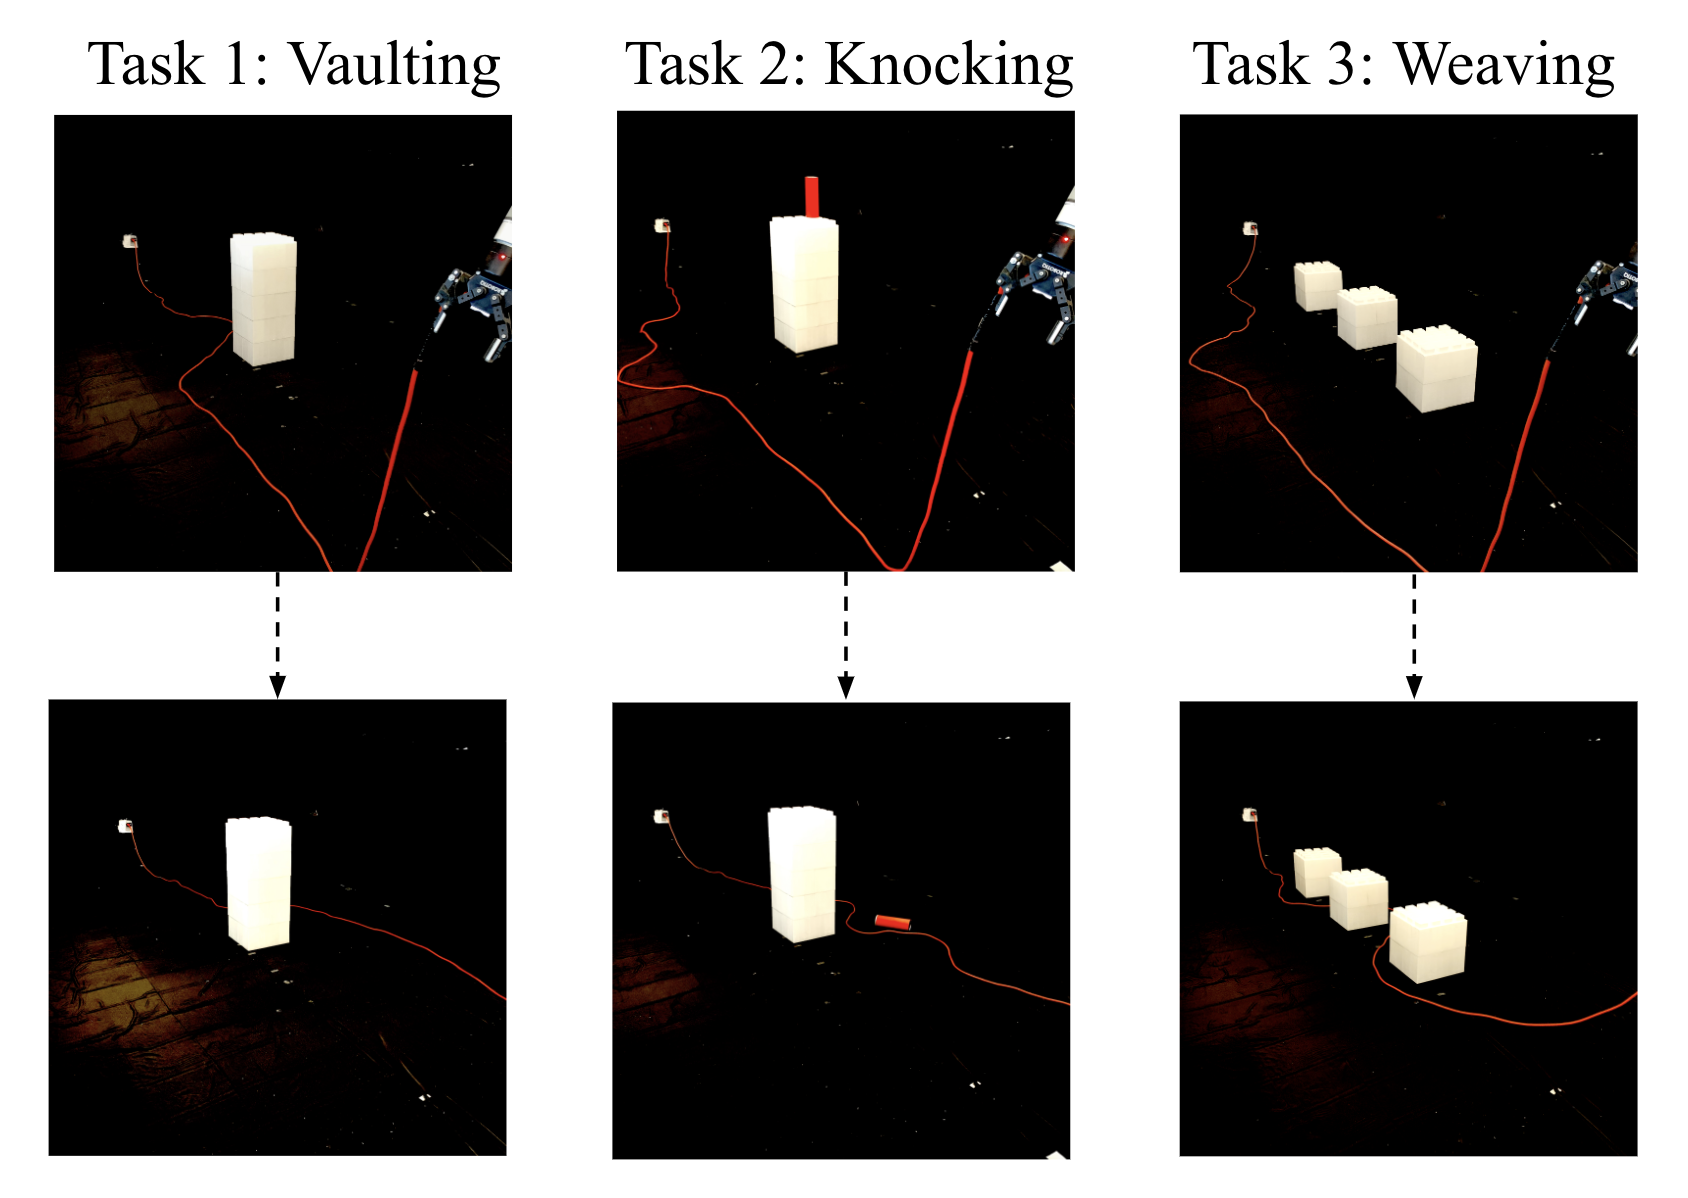
\includegraphics[width=0.48\textwidth]{figures/teaser1.png}
\begin{tikzpicture}[
every node/.style={outer sep=0,node distance=0pt,inner sep=0},
arr/.style={-latex,line width=1pt}]
% IEEE conference format: column width = 3.4in = 244.8pt
% 3 pictures * 80pt = 240pt
% (244.8 - 240)/2 = 4.8/2 = 2.4pt = spacing between pictures
% \node [options] (name) {LaTex Contents of Node};


% \draw [-Triangle,thick] (from_name) -- (to_name); 
% "-Latex" and "-triangle" are arrow types
\node (vs) {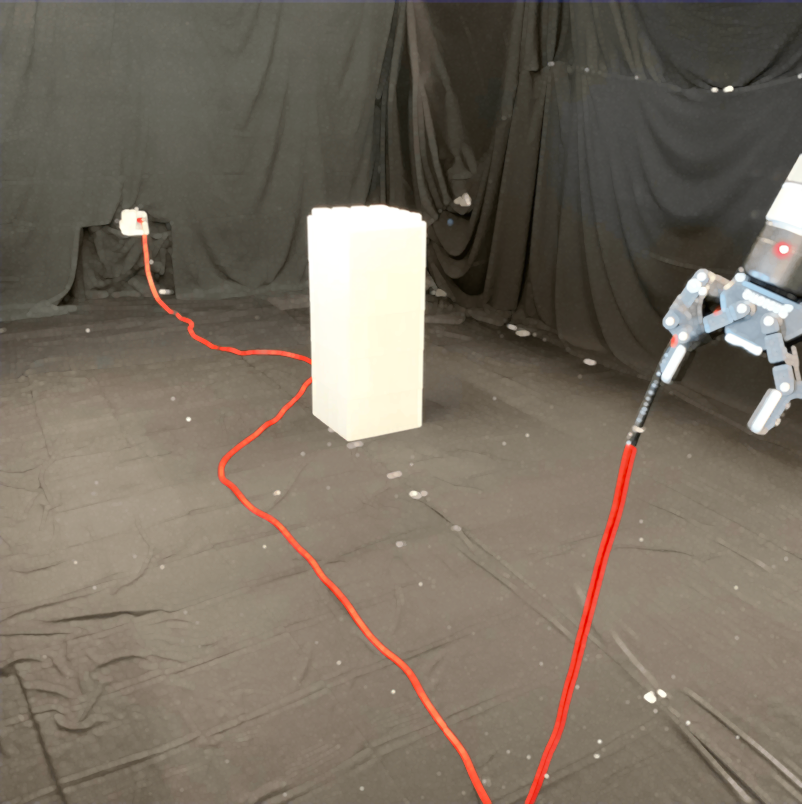
\includegraphics[width=80pt]{figures/teaser_vaulting_start.png}};
\node [right=2.4pt of vs] (ks) {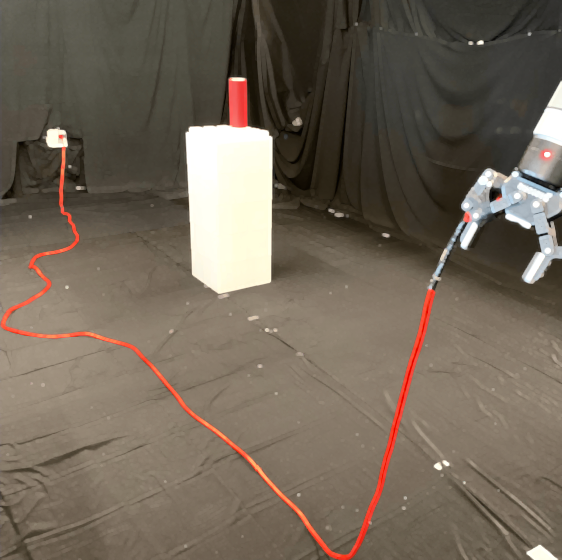
\includegraphics[width=80pt]{figures/teaser_knocking_start.png}};
\node [right=2.4pt of ks] (ws) {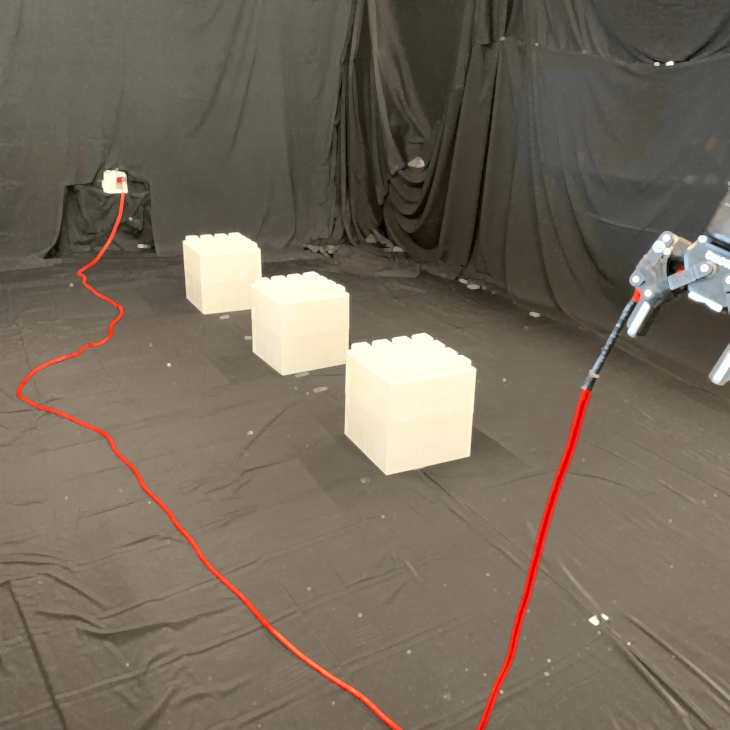
\includegraphics[width=80pt]{figures/teaser_weaving_start.png}};
\node [below=12pt of vs] (ve) {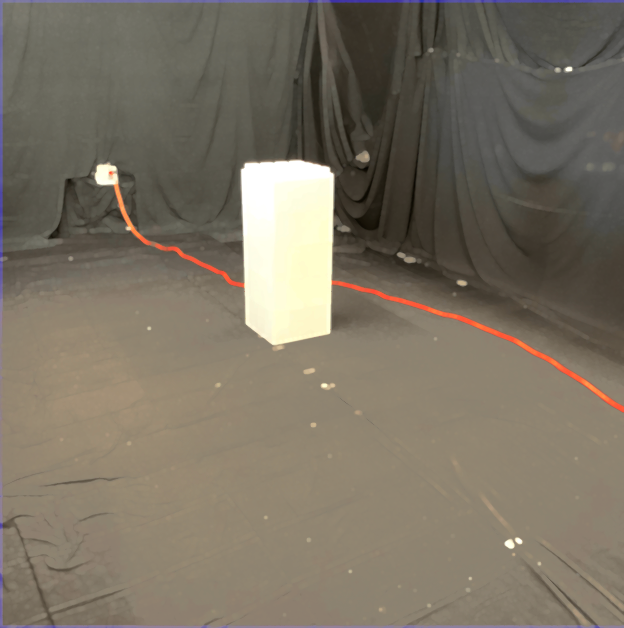
\includegraphics[width=80pt]{figures/teaser_vaulting_end.png}};
\node [below=12pt of ks] (ke) {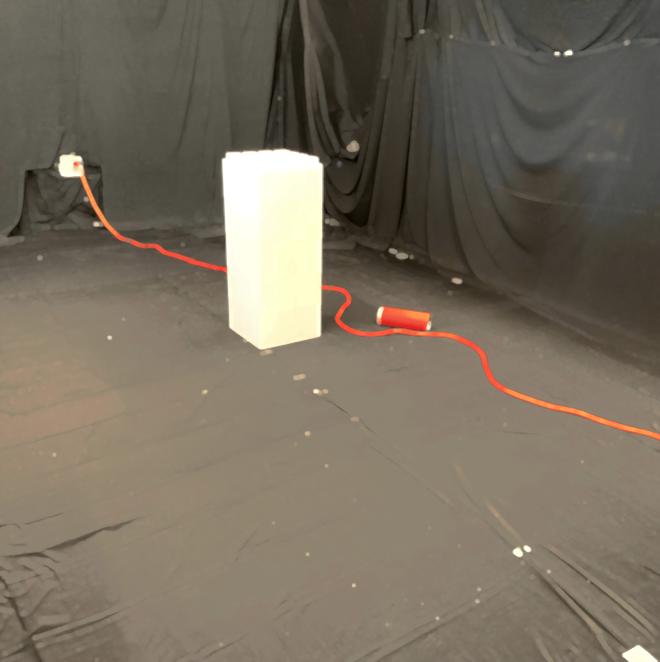
\includegraphics[width=80pt]{figures/teaser_knocking_end.png}};
\node [below=12pt of ws] (we) {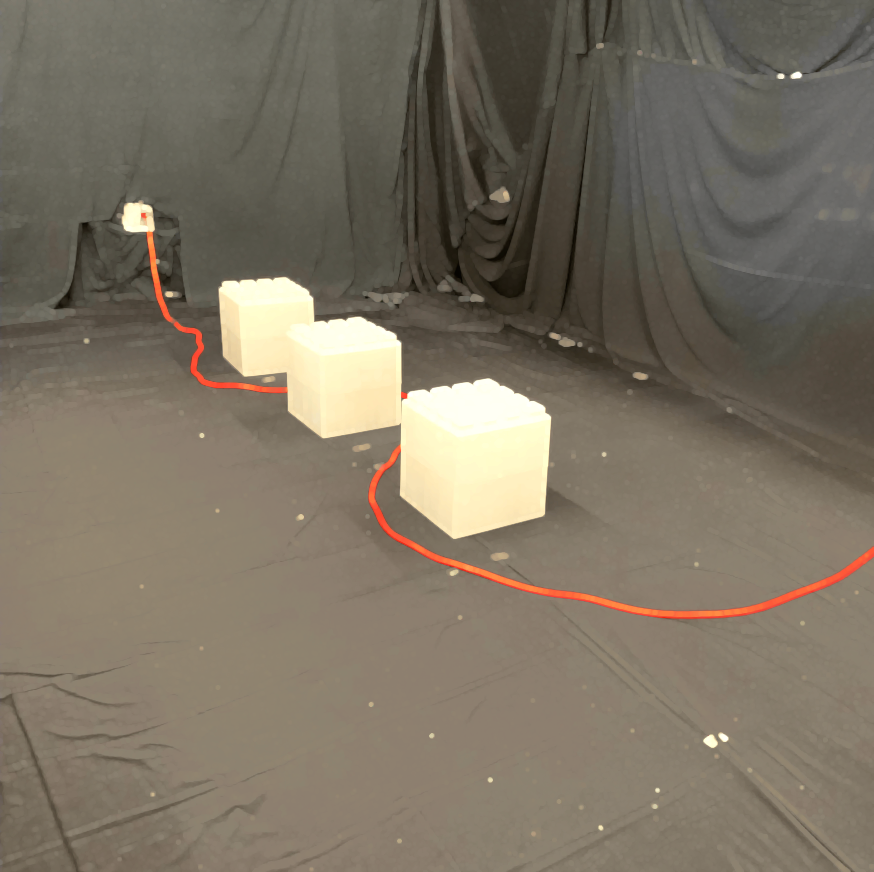
\includegraphics[width=80pt]{figures/teaser_weaving_end.png}};
\draw [arr] (vs) -- (ve);
\draw [arr] (ks) -- (ke);
\draw [arr] (ws) -- (we);
\node [below=4pt of ve] {\footnotesize (a) Task 1: Vaulting};
\node [below=4pt of ke] {\footnotesize (b) Task 2: Knocking};
\node [below=4pt of we] {\footnotesize (c) Task 3: Weaving};
\end{tikzpicture}
\caption{
\small
Illustration of the 3 tasks: Vaulting, Knocking, and Weaving in real experiments with an orange 18-gauge cable. %The cable is plugged into the wall on one end, and attached to the robot's gripper on the other end.
}
\vspace*{-15pt}
\label{fig:three_tasks}
\end{figure}

%Let $a \in \mathcal{A}$ be the action the manipulator arm takes.  Let $f_\mathcal{S}: \mathcal{S} \times \mathcal{A} \rightarrow \mathcal{S}$ be stochastic state transition function of the cable. As $\mathcal{S}$ is the infinite-dimensional configuration space of the cable, we instead rely on observations $o \in \mathcal{O}$ of the cable to define the start and goal state of the problem. Let $f_c : \mathcal{S} \rightarrow \mathcal{O}$ be a function that maps the cable's state to an observation of that state (e.g., via a camera view).  Let $T$ be the horizon of our control problem. Let $f_\mathcal{S} : \mathcal{S} \times \mathcal{A}^{T} \rightarrow \mathcal{S}$ be the stochastic open-loop state transition function of the cable after applying an actions sequence of length $T$.
%We denote states as $s_t$, observations as $o_t$, and actions as $a_t$. We denote the unknown, stochastic state transition function of the rope object as $f(s_t, a_t)$.



Since the action space $\mathcal{A}$ is also infinite-dimensional, we define a parametric trajectory function $f_{\mathcal{A}_i} : \mathbb{R}^3 \rightarrow \mathcal{A}$, that, when given an apex point, computes complete arm trajectory. While the exact function is a design choice,
we propose that the function should have
the following features: the arm motions are fast enough to induce a motion over the length of the cable, the apex point of the motion can be varied based on an $\mathbb{R}^3$ input,  the other points in the trajectory vary smoothly through the apex, and the motions are kinematically and dynamically feasible. This converts the problem to learning $\hat\pi_i : \mathcal{O} \rightarrow \mathbb{R}^3$, where $\mathcal{O}$ contains position and dimension information, such that for the action $a \in \mathbb{R}^3$ computed by the policy, $f_c(f_\mathcal{S}(s_0, f_{A_i}(a))) \in \mathcal{O}_\mathrm{goal}$.


% This is now stated in the first paragraph of the problem definition:
%We assume the manipulator arm's end-effector holds one end of the LDO, and the other end of the LDO is fixed (e.g., a power cord is plugged into the wall).
%For this work, we do not consider state feedback, and instead focus on the computation of an open-loop motion for the manipulator arm.%, so the learned policy is a shooting-method-based policy. 

% Given the initial configuration of the cable $s^r_0$ and the obstacle configuration $s^o_0$, the robot observes $o_0 = f_c( s^r_0, s^o_0 )$.
% For each task, we are given a goal set of terminal configurations $\mathcal{S}_g \subset \mathcal{S}$. For example, in the snapping task, $\mathcal{S}_g$ is a set of final configurations of the cable that knock the object over by snapping it. Therefore, we use $o_0$ and $\mathcal{S}_g$ as the input to the system. We wish to learn a policy $\pi_\theta$ such that: \harry{TODO: prof. G said Sg does not need to be specified. How do we fix this?}
% \[
% s^r_T = f_{\mathcal{S}}(s^r_0, a_{0:T-1}\sim \pi_\theta(a|o_0))\in \mathcal{S}_g
% \]
% \[
% \exists s^r_i \in \{s^r_0, ..., s^r_T\}, s^r_i = s_g
% \]
% where $s_g$ is varied for each task. For example, in the snapping task, $s_g$ is a state where the cable intersects the target object.
% In the system, policy $\pi_\theta$ is a stochastic policy that outputs a vector representing joint angles of the robot, so we are not inferring the whole trajectory of the motion, but learning a low-dimensional parameterization of a trajectory.
% %\jeffi{This is sort of previewing that we are not learning a trajectory, but a low-dimensional parameterization of a trajectory.  We may wish to be explicit on this point here.  I think though, its belongs more to the method description.} \harry{Added}
% \harry{TODO: Need to update the equation above to show that we apply this action T times.}
% Daniel: figure should take up the full width to be clearer to readers.
% \usepackage{subcaption}
% \begin{figure}[H]
% \begin{subfigure}{.25\textwidth}
%   \centering
%   % include first image
%   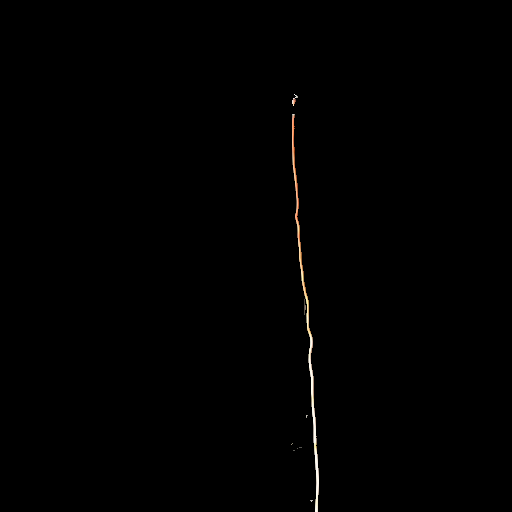
\includegraphics[width=.6\linewidth]{figures/taut_seg.png}  
%   \caption{Taut rope after reset}
%   \label{fig:sub-first}
% \end{subfigure}
% \begin{subfigure}{.25\textwidth}
%   \centering
%   % include second image
%   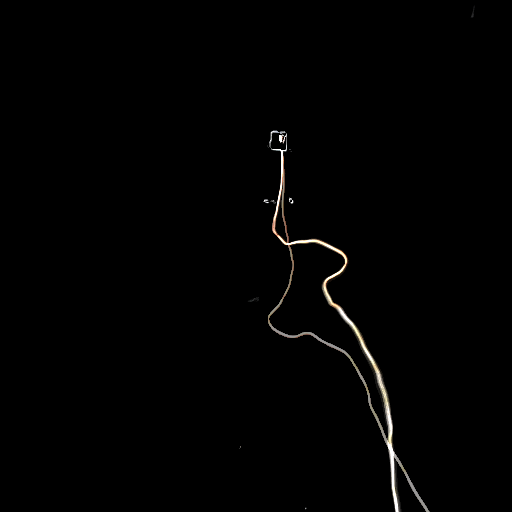
\includegraphics[width=.6\linewidth]{figures/repeat2.png}  
%   \caption{Repeatability across 20 trials}
%   \label{fig:sub-second}
% \end{subfigure}
% \caption{\textbf{Left: }the starting state of the rope is almost straight after being reset before each action begins. \textbf{Right: }overlaid image of 20 ending states of the rope after applying the same left-to-right whipping motion for 20 times given the same reset. The ending states of the rope are almost identical across 20 trials, with 1 outlier, so each action is repeatable. \harry{TODO: Re: Yes they are extremely similar. There is a kinda blurry region in the middle tho, and I did 10 more trials and had one outlier.} \jeffi{Random idea: Would it be possible to have each trial have a different color?  So we would see sort of  rainbow blob or cables?}}
% \label{fig:repeat}
% \end{figure}

\begin{figure}[t]
    \vspace*{5pt}
    \centering
    % \begin{tabular}{c@{\hspace{1.5pt}}c@{\hspace{1.5pt}}}
    %\subfloat[Ending states without reset]{%
    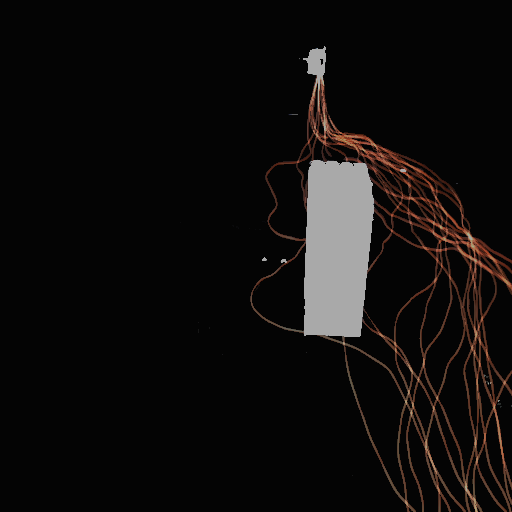
\includegraphics[height=122pt]{figures/unrepeata.png}%}%
    \hfill
    %\subfloat[Ending states with reset]{%
    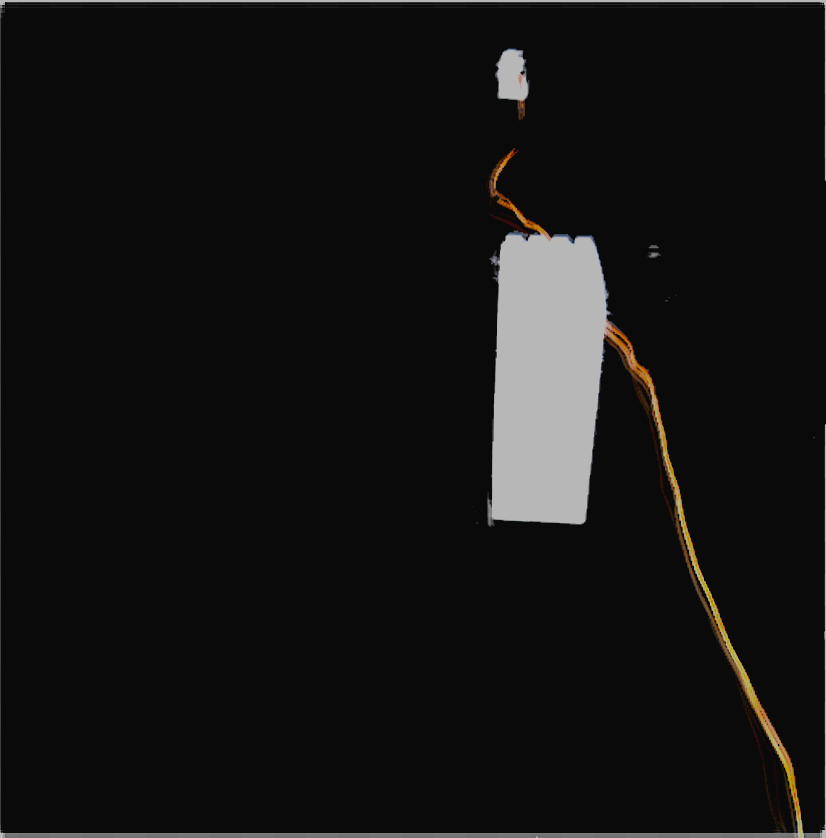
\includegraphics[height=122pt]{figures/repeat4a.png}%}
    % \end{tabular}
    \caption{\textbf{Repeatability without (left) and with (right) taut-pull reset.} 
    Both images show an overlay of 20 ending cable configurations after sequentially applying the same left-to-right vaulting trajectory 20 times. \textbf{Left: }without applying resets before the motion, there is high variation in ending configurations.  \textbf{Right: }resetting the cable via a taut-pull before the motion results in nearly identical configurations across 20 left-to-right attempts.}% The vaulting actions are surprisingly repeatable with reset.}
    %\vspace*{-10pt}
    \label{fig:repeat}
\end{figure}

